\section{London Congestion Charge}\label{sec:london}

\subsection{Implementation}

Concrete steps towards a scheme finally began in 1997, when the UK's new Labour government called a referendum on the question of creating a Greater London Authority---a regional governing body over London's many boroughs---to be headed by an elected Mayor of London.\footnote{Except where indicated, information in this section comes from \citet[Ch. 6]{Richards2006}. See also \citet[Sec. 7.2]{TfLFifth2007} for a concise list of steps to implementation.} In May 1998, this concept won the referendum by a large margin, although it was still up to Parliament to craft specific legislation to create the GLA. Several Labour policy papers suggested the new Mayor's powers would include enacting road pricing, and so in August 1998 the Government Office for London convened a team of experts, the Road Charging Options for London (ROCOL) Working Group, to study the matter one last time. Around the same time, the UK Treasury decided that it would permit revenues from pricing to be hypothecated to transportation---a break with the usual practice whereby all British government revenues are allocated by the government. In 1999, Parliament passed the Greater London Authority Act \citep{Parliament1999}, which created the Mayor position and did give the role road pricing powers, under the proviso that the first ten years of revenue be hypothecated to transportation. 

In March 2000 ROCOL published its report, \citet{ROCOL2000}, and in May 2000, the first mayoral election went to Ken Livingstone, who had included DCP in his election manifesto (campaign platform). After being briefed on \citet{ROCOL2000}, Livingstone decided to move forward with enforcement by Automatic Number Plate Recognition (ANPR) cameras---a technology perfected in the 1990s. ROCOL had also considered paper licenses and tag-and-beacon systems, but cautioned that the former were impractical and the latter would mean delaying the scheme beyond the Mayor's first term, since national authorities were still working on national standards for transponders. ANPR has the advantage that vehicles do not have to carry special equipment, and has been used in every DCP system except Singapore's.

After preparation and consultation with the public in which several features of the ROCOL plan were modified (e.g., eliminating a proposed higher rate for goods vehicles, granting discounts to residents of the charging zone) the London Congestion Charge went into effect on February 17th, 2003. The launch of the scheme was supported by a permanent expansion of bus service as well as roadwork and traffic signal changes designed to mute the impact of traffic on nearby untolled areas---as described in \cite[p. 132-135]{Richards2006}.

\subsection{Design}

The LCC launched as a \pounds5 charge for unlimited travel between 7:00 AM and 6:30 PM within the 22 km$^{2}$ Congestion Charging Zone (CCZ) (the solid region in Fig. \ref{fig:London-Congestion-Charging}). The zone is surrounded by the capacious, uncharged Inner Ring Road which allows drivers to avoid the zone. Uniquely, the LCC covers all travel within the zone---not just traversals of a cordon like the other schemes---as well as vehicles that are merely parked on the street. Therefore, enforcement requires ANPR cameras (over 500 at the launch) mounted on poles throughout the zone and along its boundaries, as well as cameras mounted on patrolling vans. The baseline payment method is as follows: if one uses public streets in the CCZ during charging hours, one has until midnight to pay by calling a number, SMS, a website, payment machines or in various stores. The LCC is turned off from December 25th to January 1st of every years, for Christmas and New Years.

The LCC has undergone a number of minor changes of which we will list only a few. The toll was raised from \pounds5 to \pounds8 in July 2005, \pounds10 in January 2011 and \pounds11.50 in June 2014. In 2007, the end of charging was moved up from 6:30 to 6:00 PM. Since June 2006, if one pays by midnight on the day after visiting the zone the penalty is small (\pounds 2.50). Since 2011, an Auto Pay option lets users have their accounts debited automatically, whereas before this was only available to businesses participating in the ``Fleet Scheme.''

The largest, albeit temporary, change to the LCC has been the ``Western Extension,'' a 19 km$^2$ addition to the original CCZ which is shown as the striped area in Fig. \ref{fig:London-Congestion-Charging}. After Livingstone was reelected in May 2004, he carried out a consultation with the public on the Extension \citep[Ch. 14]{Richards2006}. The result was soundly negative, but Livingstone chose to proceed anyway, and the Extension came into operation on February 19, 2007. When Boris Johnson defeated Livingstone in the 2008 mayoral election, he conducted another public consultation, \citet{TfL2008b}, on the  Extension. Results showed the public still very opposed, and so the Extension was scrapped on January 4, 2011.

There are myriad exemptions and discounts. Using Auto Pay earns a \pounds1 discount. Residents receive a 90\% discount. Motorcycles, buses, vehicles with 9+ seats, licensed taxis/minicabs, certain emergency and government vehicles, certain vehicles used for or by  disabled people, and certain vehicles with very low emissions are all completely exempt or eligible for a ``100\% discount,'' which, unlike exemption, requires registration and possibly a small fee. The difference between a taxi and minicab is that taxis (also called ``black cabs'') are special black-colored cars that can be hailed from the street, whereas minicabs (also called ``private hire vehicles'') are ordinary cars that can only execute pre-booked pickups. Below, minicabs and private cars are grouped together in statistics---even though the former are exempt---because they are visually indistinguishible from private cars. Finally, travelers getting care at National Health Service facilities can be reimbursed for the charge.

\begin{figure}[ht]
    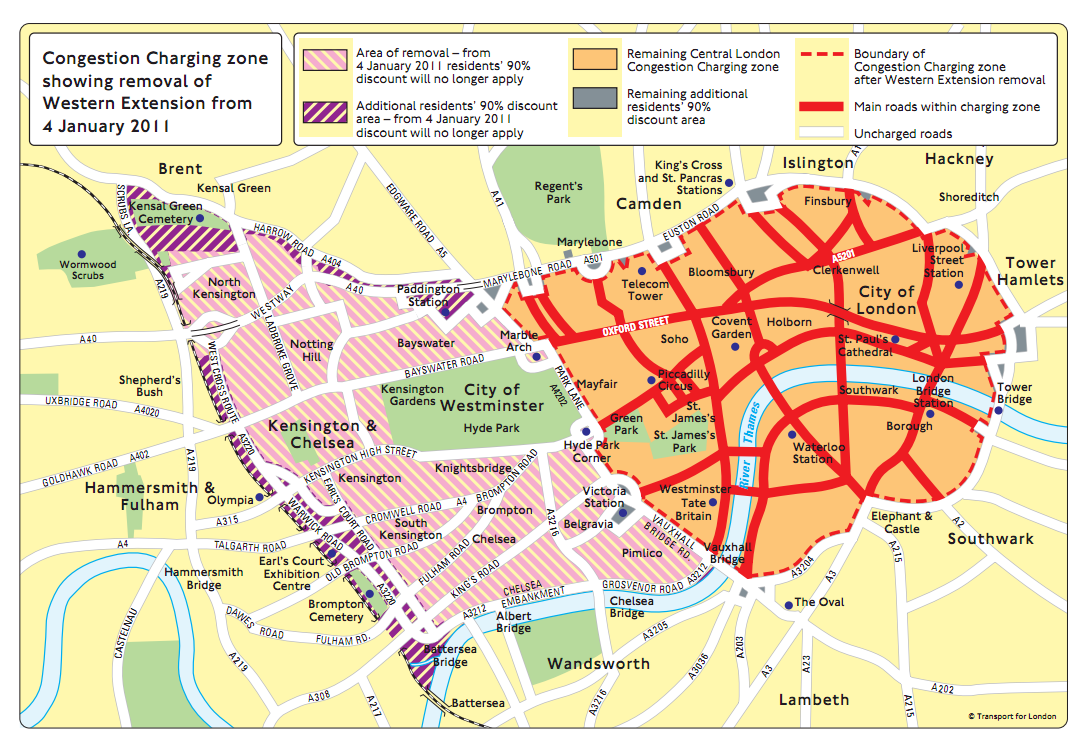
\includegraphics[width=1\textwidth]{../img/london-congestion-charge.png}
    
    \caption{London Congestion Charging Zone \label{fig:London-Congestion-Charging}}
\end{figure}


\subsection{Transportation impacts}

The LCC is the most closely studied DCP system. Transport for London (TfL) collected data on traffic, travel times, business, transit use and other impacts of the Congestion Charge under the Impacts Monitoring Programme, described in \citet[Sec. 1]{TfLFirst2003}. Findings appear in annual reports from 2003 to 2008, after which more limited data can be found in the TfL's annual Travel in London Report.

The most significant accomplishment of the LCC has beeen to reduce entries to the CCZ and to recompose traffic. See  \ref{fig:london-entries} for entries to the CCZ between 2002 and the first five years of charging. From 2002 to 2003 (before and after the charge), entries by cars and minicabs fell by 33\% (65k) and entries by all potentially-chargeable vehicles (cars/minicabs, trucks and vans) fell 27\% (73k) \citep[p. 22, Tab. 2.2]{TfLFifth2007}. The effect on chargeable traffic was offset by an 18\% (10k) surge in taxi traffic, for a net 18\% fall in entries by all vehicles with 4+ wheels. These patterns held steady through 2007 \citet[p. 41, Tab. 3.1]{TfLSixth2008}. \citet{TfL2017} reports that recent years have seen a steep rise in exempt private hire vehicles, caused by Uber. In response, news reports suggest that London's current Mayor, Sadiq Kahn, is considering removing the minicabs' exemption.
% \footnote{https://www.thetimes.co.uk/article/london-congestion-charge-on-minicabs-to-boost-buses-5kkbqprg9}

% Illustrating Theme II, \citet{TfLDemand2008} note that 


Illustrating Theme II, \citet[p. 19]{TfLFifth2007} remarks, ``Of particular note is the relatively indistinct response to the increase to the daily charge [from \pounds 5 to \pounds 8] in July 2005.'' The next year, TfL published a report on price elasticity noting that the elasticity of demand implied by the toll increase was only -0.16, whereas that implied by the original \pounds 5 toll was -0.51 \citep{TfLDemand2008}.

Results for speed have been more disappointing. (Note first that TfL reports speed changes in terms of the inverse measure min/km, which traffic engineers sometimes call ``pace.'') Before charging, the average pace in the CCZ during charging hours was 4.1 min/km (14.6 kph); in 2003 and 2004 pace fell to about 3.4 min/km (17.6 kph) \citep[Sec. 3.4]{TfLFifth2007}. TfL assumes a baseline, uncongested pace of 1.8 min/km, and so the delay attributed to congestion fell by 30\%. As soon as 2007, however, pace had reverted to its pre-charging level \citep[Sec. 4.4]{TfLSixth2008}. The traffic data firm INRIX reports that, from 2012 to 2015 (inclusive), pace in the CCZ rose by 22\% (i.e., speed fell by 19\%) \citep{INRIX2016}.

TfL has blames falling speed to road work and to capacity-reducing projects such as bus lanes, bus priority and pedestrian or cycling safety measures. The evidence is that similar falls in speed---adjusted for flows---have happened outside the CCZ and at night \citep[Sec. 3.11]{TfLFifth2007}. \citet[p.3]{TfLExPost2007} raises an interesting possibility: ``It is probable that some of these [capacity reallocation] measures have been enabled by charging and would not have happened had charging not reduced traffic levels in the centre of London.'' In this case, the LCC can be looked at not as a way to \emph{raise} traffic speeds but rather as a way to \emph{maintain} traffic speeds while obtaining other public goods and more construction. 

By comparing trends in London against other British cities, \citet{Green2016} find the LCC reduced the number of car accidents per month by 35\%, with the fall explained by both less traffic flow and 22\% fewer accidents per million km-traveled. Areas surrounding the zone exhibited declines as well.

The LCC seems to have boosted bus ridership, although in the long run it is hard to say by how much given that London's bus system has been substantially improved.  From 2002 to 2003, 38\% more bus riders entered the CCZ during the morning; \citet[pp. 40-41]{TfL2004a} attributes half that change to charging and half the bus improvements. \citet[p. 55]{TfL2004a} estimates that, of the 65k car trips diverted between 2002 and 2003, about half switched to bus. In the first year of charging, there was no increase in metro ridership. 

\begin{figure}[ht]
    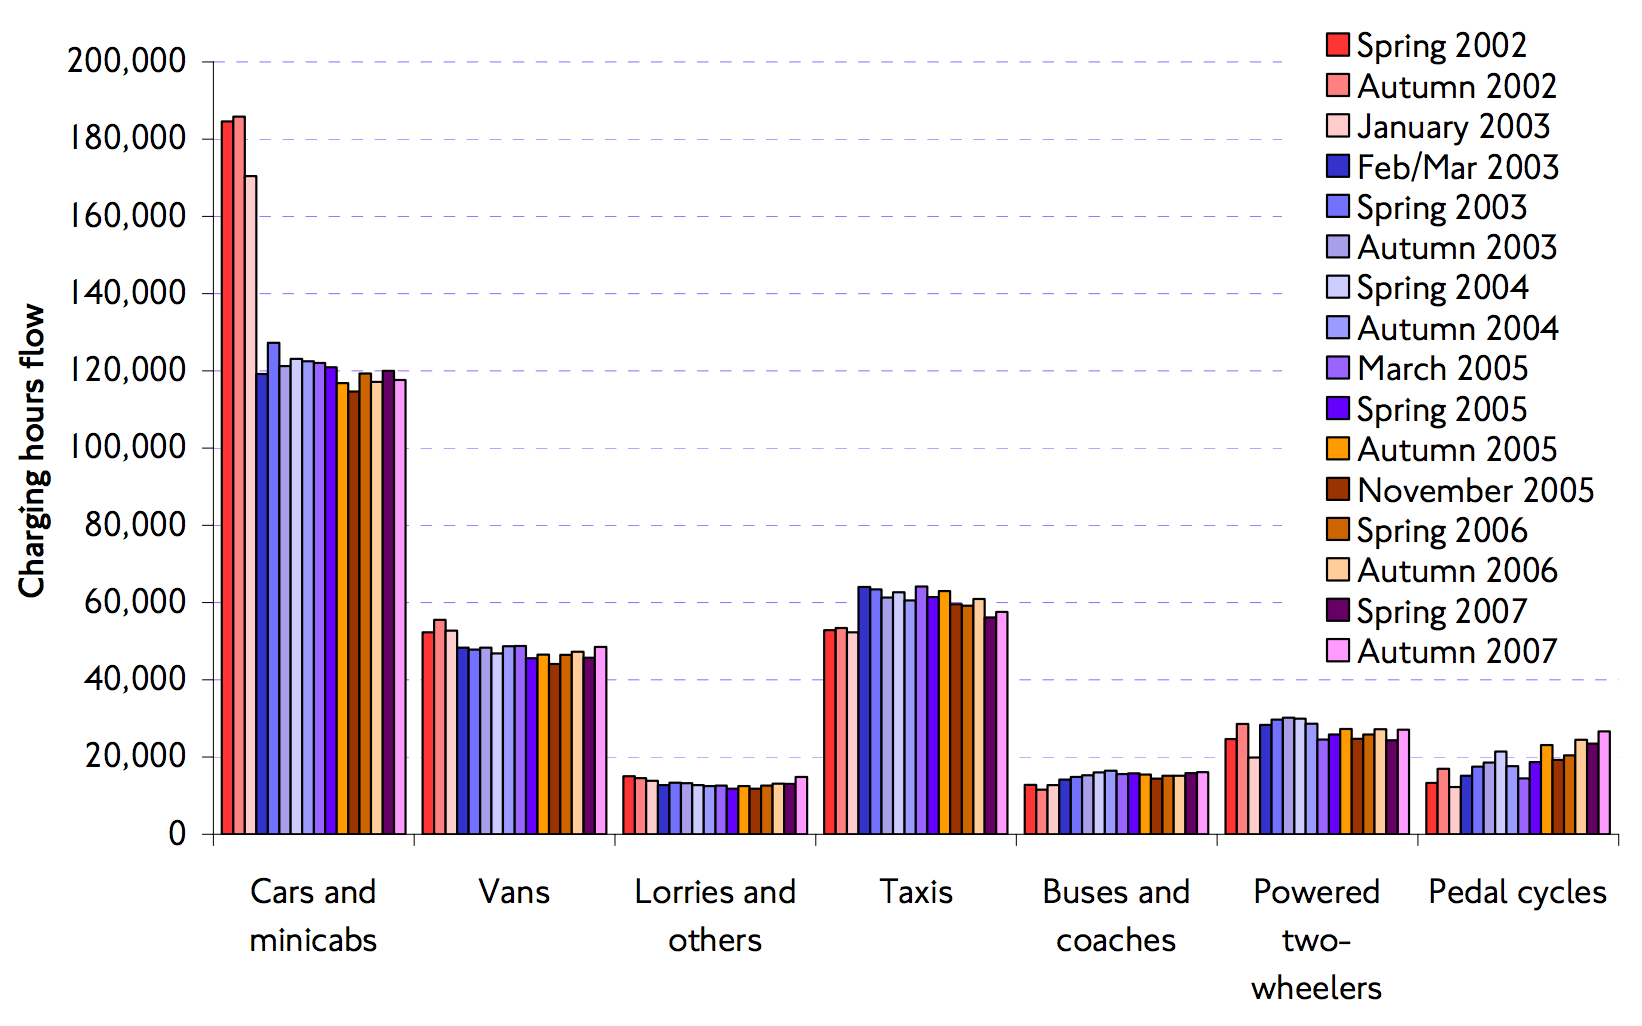
\includegraphics[width=.95\textwidth]{../img/london-entries.png}
    \caption{Entries to the original LCC charging zone by traffic type. \citep[p. 20]{TfLFifth2007} } \label{fig:london-entries}
\end{figure}

\subsection{Finances}
Financially, the LCC has cost more to build and operate and generated, until recently, less money than expected.

\citet[p. 125]{ROCOL2000} predicted setup costs of \pounds30-50 million. In reality, TfL reported implementation costs of \pounds162 million \citep[p. 135]{TfLFifth2007}, but this number requires some context: about \pounds 100 million paid for traffic management measures, including projects for cyclists and pedestrians, bus priority, better signal timing and road improvements \citep[pp. 132-133,138]{Richards2006}. While the LCC may have been the impetus behind these projects, arguably they produced auxiliary own benefits or were to some degree optional. At the same time, this amount does not include the costs of additional public transit provision that went along with the scheme.

As for the yearly budget, \citet{ROCOL2000} estimated annual revenues of \pounds 260-320 million (\pounds 230-270 million from charges and \pounds 30-40 million from penalties) and operating costs of \pounds 30-50 million. ROCOL's plan, however, did not include exemptions for residents or taxis/private hire vehicles; and it imposed a higher charge on delivery vans and trucks. Taking the changes and more realistic costs into account, \citet{TfL2002} projected net revenues of \pounds 130-150 million, not counting penalties. In reality, operating costs have been much higher and revenues lower, as shown in Table \ref{tab:London-Congestion-Charge}. The Impacts Monitoring reports break down revenue allocation, showing the vast majority went to bus service, with smaller amounts for roadworks, safety, walking/cycling measures and other uses. Costs and revenues seem to have stabilized at around \pounds 90 and \pounds 250 million, respecitvely, leading to surpluses of around \pounds 160 million.

\citet[p. 186]{TfL2003b} attributed the shortfall in revenue, initially, to evasion, a greater-than-expected fall in chargeable traffic and the large share of exempt traffic. In 2007, TfL noted that only 44\% of entering vehicles with 4+ wheels were subject to full charge \citep[p. 12]{TfLExPost2007}. Almost as many, 38\%, were made by exempt taxis and private hire vehicles or discounted residents. 

\begin{table}[ht]
    \begin{tabular}{|c|c|c|c|c|c|c|}
        \hline 
        financial year & price & charges & penalties & revenue & cost & net revenue\tabularnewline
        \hline 
        \hline 
        02/03 & 5 & 18 & 1 & 19 & 17 & 2\tabularnewline
        \hline 
        03/04 & 5  & 116 & 55 & 171 & 93 & 78\tabularnewline
        \hline 
        04/05 & 5 & 117 & 75 & 192 & 90 & 102\tabularnewline
        \hline 
        05/06 & 5/8 & 144 & 66 & 210 & 88 & 122\tabularnewline
        \hline 
        06/07 & 8 & 158 & 55 & 213 & 90 & 123\tabularnewline
        \hline 
        07/08{*} & 8 & 195 & 73 & 268 & 131 & 137\tabularnewline
        \hline
        08/09* & 8 & - & - & 326 & 177 & 149\tabularnewline
        \hline 
        09/10* & 8 & - & - & 313 & 154 & 158 \tabularnewline
        \hline 
        10/11* & 8/10 & - & - & 287 & 113 & 174\tabularnewline
        \hline 
        11/12 & 10 & - & - & 227 & 90 & 137\tabularnewline
        \hline 
        12/13 & 10 &  - & - & 222 & 90 & 132\tabularnewline
        \hline 
        13/14 & 10 & - & - & 235 & 85 & 149\tabularnewline
        \hline 
        14/15 & 11.5 & - & - & 257 & 85 & 173\tabularnewline
        \hline 
        15/16 & 11.5 & - & - & 258 & 90 & 168\tabularnewline
        \hline 
        16/17 & 11.5 & - & - & 250 & 86 & 164\tabularnewline
        \hline 
    \end{tabular}
    
    \caption{London Congestion Charge costs and revenues. Starred years are those when the Western Extension was in force. The financial year runs from April 1st through March 31st. 2003-2008 data from TfL's \emph{Congestion Charging Monitoring} reports. Later data from TfL's Annual Reports \citep{TfL2018} }\label{tab:London-Congestion-Charge}
\end{table}